%!TEX root = thesis.tex

\chapter{Methoden} % (fold)
\label{cha:methoden}

\section{Graphen} % (fold)
\label{sec:graphen}
Da die Breitensuche ein asymptotisch relativ schneller Algorithmus ist, sind relativ große Testgraphen nötig, um einigermaßen aussagekräftige Ergebnisse zu erhalten. Für diese Arbeit wurden Graphen in der Größenordnung von 100 000 Knoten gewählt. Diese wiederum relativ kleine Ausdehnung wurde gewählt, da der Testmodus unter anderem beinhaltet, dass bei gleichbleibender Knotenanzahl die Dichte des Graphen variiert. Sehr dicht besiedelte Graphen mit 100 000 Knoten passen gerade noch in den Arbeitsspeicher. Würden noch größere Graphen verwendet, müsste entweder die Dichte des Graphen beschränkt werden oder das Betriebssysteme müsste Speicherseiten auslagern, was die Messergebnisse unbrauchbar machen würde. Da die asymptotische Laufzeit der Breitensuche aber O(n + m) ist \cite{SWB-283374373}, wäre eigentlich zu erwarten gewesen, dass bei gleicher (absoluter) Kantenzahl und erhöhter Knotenzahl, die Laufzeit nur leicht erhöht ist. Ein Beispiel: BFS auf einem Graph mit 1 000 000 Knoten und durchschnittlichem Knotengrad von 100 (ergibt 100 Mio Kanten) sollte kaum länger dauern, als die BFS auf einem Graph mit 100 000 Knoten und durchschnittlichem Knotengrad von 1000 (ergibt ebenso 100 Mio Kanten). Diese Annahme ist für den parallelen Fall falsch, da die zu versendenden Datenmengen erheblich größer werden, wenn der Graph mehr Knoten hat.

Es wurde ein Tool namens graph-generator \cite{graph-generator:2009:Online} eingesetzt, um zufällige Graphen zu generieren. Um einen Graph zu erstellen, müssen folgende Parameter gewählt werden:
\begin{enumerate}
	\item Die Anzahl an Knoten.
	\item Der minimale Ausgangsgrad jedes Knotens.
	\item Der maximale Ausgangsgrad jedes Knotens.
	\item Der Exponent der Exponentialverteiltung. Es wurde immer 5 gewählt.
	\item Der mittlerer Knotengrad z.
\end{enumerate}
Der Ausgangsgrad der Knoten ist folgendermaßen verteilt:
$$
P(X=k) \propto (k + offset)^{-exp}
$$
Der Offset wird dabei automatisch von dem Tool derart gewählt, dass sich ein durchschnittlicher Ausgangsgrad von z ergibt.
% section graphen (end)

\section{Testplattform} % (fold)
\label{sec:testplattform}
Als Testplattform kann ein Apple Notebook von 2011 zum Einsatz. Es hat einen Intel Core i7-2720QM \enquote{Sandy Bridge} Prozessor, der mit 2.2Ghz getaktet wird. Es stehen 4 physikalische Kerne zur Verfügung, die jeweils Intels Hyper Threading Technologie unterstützen. Dadurch sind physikalisch 8 parallel laufende Threads möglich. Beim Vergleich von sequentiellen Algorithmen mit parallelen ist zu beachten, dass der Prozessor einen Kern auf bis zu 3.3 GHz übertakten kann, falls die anderen Kerne momentan nicht verwendet werden. Der optimal erreichbare Speedup ist demnach nicht 8.0, sondern deutlich darunter. Das Testsystem ist außerdem mit 8GB Hauptspeicher ausgestattet, der bei einem Takt von 1333Mhz arbeitet. Auf dem Testsystem wird als Betriebssystem Mac OS X 10.6.8 \enquote{Snow Leopard} und der x10 Compiler in der Version 2.2.3 verwendet.
% section testplattform (end)

\section{Modus} % (fold)
\label{sec:modus}
Um Ergebnisse aus je einer Algorithmus - Graph - Kombination zu erhalten, wird der gewählte Algorithmus drei mal auf dem gewählten Graph ausgeführt und die Zeit gemessen, die die reine Berechnung benötigt. Die Zeit, um den Graph in den Speicher einzulesen und die Daten auf die Places aufzuteilen, wurde nicht gemessen, da sie wenig mit dem Algorithmus oder X10 zu tun hat. Die Zeit, die benötigt wird, um das Ergebnis von den beteiligten Places zurück zum Ursprungsplace zu kopieren, wird allerdings mitgemessen.

Die X10 Laufzeitumgebung liest beim Programmstart die Umgebungsvariablen X10\_NPLACES, in der steht, wie viele Places lokal auf diesem Rechner simuliert werden sollen. Die einzelnen Places werden durch Prozesse (nicht Threads) repräsentiert, wodurch sie tatsächlich getrennte Speicherbereiche haben. Der Aufbau entspricht zwar nicht dem Optimalsetup, in dem jeder X10 Prozess auf einen physikalisch getrennten Computer operiert, doch auch der Kontextwechsel, der bei der Kommunikation zwischen Places auftritt, ist relativ langsam und somit eine Annäherung an realen Kommunikationsoverhead. Trotzdem sind diese Ergebnisse nicht eins zu eins auf einen Rechnerverbund zu übertragen. Das liegt zum einen daran, dass, wie gesagt, die Kommunikation nochmal erheblich teurer wird, zum anderen können mit einem Rechnerverbund wesentlich größere Graphen bearbeitet werden, die offensichtlich ein viel höheres Potential zur Parallelisierung bieten. Andererseits dürfen die Ergebnisse dieser Arbeit auch nicht mit der lokalen Parallelisierung der Breitensuche auf einem einzelnen Rechner verwechselt werden. Kommunikation mittels geteiltem Speicher ist deutlich schneller, als die hier verwendete Inter-Prozess-Kommunikation. Es sei hier auch nochmal darauf hingewiesen, dass pro Prozess, also pro Place, immer nur ein Thread aktiv ist.
Um die Möglichkeit der Parallelität zu messen, wurde der Algorithmus in der 1D und der 2D Zerlegung jeweils in einer Konfiguration mit 1, 2, 4, 8 und 9 Places ausgeführt. Die Konfiguration mit 9 Places wurden hinzugenommen, da so bei der 2D Zerlegung eine symmetrische 3 mal 3 Zerlegung stattfinden kann. Es wurde vermutet, dass eine quadratische Anzahl an Places besonders günstig für diesen Algorithmus sind, obwohl 9 Places mehr sind, als Rechenkerne zur Verfügung stehen. Der Vollständigkeit halber wurde auch der 1D Algorithmus mit 9 Places durchgeführt. Um wirklich vollständige Ergebnisse zu bekommen, sollte eigentlich pro Graph die Breitensuche einmal von jedem Knoten aus gestartet werden. Allein diese Unterfangen würde den Zeitrahmen der kompletten Arbeit sprengen.

Der Modus, mit nur einem Thread pro Place und ohne die Nutztung von geteilten Speicher zwischen den einzelnen Ausführungsfäden lässt neben der Übertragbarkein auf die invasive Hardware auch Rückschlusse auf Manycore - Systeme zu. Bei diesen CPUs der Zukunft sollen viele kleine Rechenkerne auf einer CPU platziert sein. Cachekohärenz mit geteiltem Speicher ist dann kaum noch möglich. Auch wird jeder Kern nur einen Ausführungsfaden gleichzeitig bearbeiten können. Die hier vorgeschlagenen Implementierungen sind also für solch eine Hardware interessant.
% section modus (end)

\chapter{Ergebnisse und Diskussion} % (fold)
\label{cha:ergebnisse_und_diskussion}

Die vollständigen Messergebnisse finden sich in den Anhängen \ref{Anhang-Messwerte-Dichte}, \ref{Anhang-Messwerte-Verteilung} und \ref{Anhang-Messwerte-Groesse}. Es wurden die Auswirkungen der Variation der Dichte, der Knotenzahl und der Verteilung des Graphen auf die Laufzeit gemessen, wobei jeweils die anderen Parameter fest gewählt waren. Sehr dünn besetzte und kleine Graphen waren deutlich schneller mit einer seriellen Version der Breitensuche zu lösen, als es mit jedwedem parallelen Algorithmus möglich war. Der Vergleich der seriellen Breitensuche, mit der 1D-Breitensuche mit einem Place ist durchaus auch interessant und wird in Kapitel \ref{sec:serieller_fall_vs_1d_mit_einem_place} vertieft. Der 2D-Algorithmus schnitt in allen Testfällen dermaßen schlecht ab, dass er gesondert in Kapitel \ref{sec:die_2d_breitensuche} behandelt wird.

\section{Serieller Fall, 1D mit einem Place und 2D mit einem Place} % (fold)
\label{sec:serieller_fall_vs_1d_mit_einem_place}
Jeder Algorithmus muss pro Iteration jeden aktiven Knoten mindestens einmal anfassen. Außerdem muss jeder Algorithmus pro Iteration jeden der Knoten mindestens einmal anfassen, der von einem der aktiven Knoten aus erreichbar ist. Der serielle Algorithmus tut genau das und nicht mehr. In Tests wurde herausgefunden, dass eine Iteration mittels einer herkömmlichen for-Schleife mit anschließendem direkten Elementzugriff über den Index deutlich schneller ist, als eine foreach-Schleife. Der 1D-Algorithmus muss pro Iteration die Knoten in Sendepuffer einsortieren (jeden aktiven Knoten einmal anfassen) und verschicken, was im Fall mit nur einem Place aber eine einfache Zeigerzuweisung ist. Anschließend muss dann nochmals jeder aktive Knoten angefasst werden, um alle erreichbaren Knoten zu erhalten. Der 1D-Algorithmus muss also zweimal über alle aktiven Knoten iterieren, zumindest in einer naiven Implementierung. Die verwendete optimierte Version legt diese beide Phasen aber zusammen. Zusätzliche Arbeit, im Gegensatz zu der seriellen Version, hat der 1D Algorithmus also nur beim Zurückkopieren des gesamten BFS-Distanz-Arrays. Die Messergebnisse zeigen, dass der serielle Algorithmus für recht dichte Graphen langsamer ist, als der 1D Algorithmus, wenn er mit nur einem Place gestartet wird. Nur bei sehr dünn besetzten Graphen ist die Laufzeiten des seriellen Algorithmus ein Wenig schneller. Die Messergebniss zur Variation der Größe zeigen ebenfalls, dass auch bei großer Knotenzahl der serielle Algorithmus der schnellste ist, solange der durchschnittliche Knotengrad nicht zu groß wird.

Wieso der serielle Algorithmus auf Listenbasis nicht der schnellste ist, wie eigentlich erwartet, ist nicht ohne weiteres zu erklären. Zufall in Verbindung mit der Garbage Collection sind in Anbetracht der Deutlichkeit der Ergebnisse auszuschließen. Eine mögliche Erklärung ist, dass der Compiler den einen Code besser optimieren konnte, als den anderen, ohne dass sofort offensichtlich ist, woran das liegt.

Wie aus Abbildung \ref{Vergleich_Seriell} hervorgeht, ist der 2D Algorithmus deutlich langsamer als die beiden anderen. Der 2D Algorithmus hat 2 Kommunikationsphasen pro Iteration. In den beiden Phasen wir aber jeweils nur mit $\sqrt(p)$ anderen Places kommuniziert (bei p Places)\cite{Buluc:2011}, während im Fall des 1D Algorithmus jeder Place potentiell mit allen anderen kommuniziert. Im seriellen Fall ist diese zusätzliche Komplexität nicht nötig, verlangsamt aber den Ablauf.
% section serieller_fall_vs_1d_mit_einem_place (end)  

\begin{figure}
	\centering
	\label{Vergleich_Seriell}
	\caption{Vergleich der Laufzeiten bei serieller Ausführung, also nur ein Place bei 1D und 2D Algorithmus, jeweils schnellste gemessene Laufzeit.}
	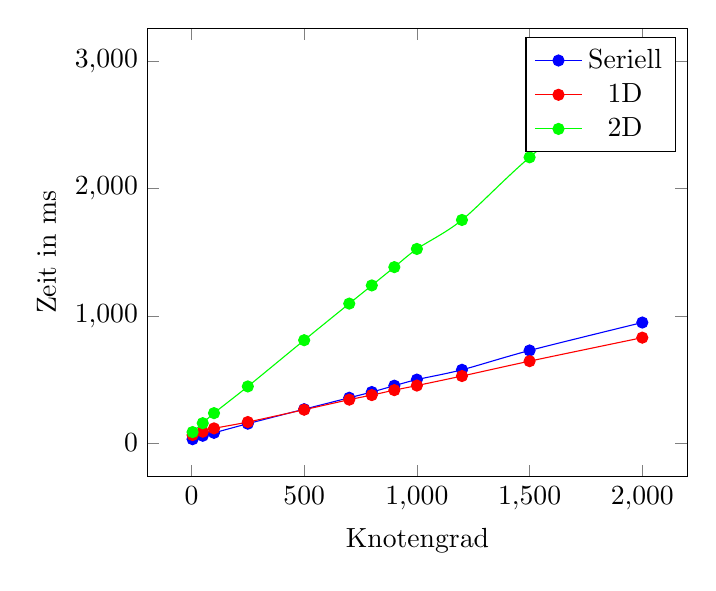
\begin{tikzpicture}
	    \begin{axis}[
	        xlabel=Knotengrad,
	        ylabel=Zeit in ms]
	    \addplot[smooth,mark=*,blue] plot coordinates {
	        (5,29)
	        (50,56)
	        (100,79)
	        (250,151)
	        (500,265)
	        (700,355)
	        (800,400)
	        (900,450)
	        (1000,498)
	        (1200,575)
	        (1500,727)
	        (2000,947)
	    };
	    \addlegendentry{Seriell}

	    \addplot[smooth,color=red,mark=*]
	        plot coordinates {
	        (5,62)
	        (50,88)
	        (100,114)
	        (250,164)
	        (500,261)
	        (700,340)
	        (800,376)
	        (900,415)
	        (1000,451)
	        (1200,526)
	        (1500,643)
	        (2000,828)
	        };
	    \addlegendentry{1D}

	    \addplot[smooth,color=green,mark=*]
	        plot coordinates {
	        (5,85)
	        (50,155)
	        (100,234)
	        (250,444)
	        (500,808)
	        (700,1096)
	        (800,1239)
	        (900,1383)
	        (1000,1526)
	        (1200,1754)
	        (1500,2247)
	        (2000, 2969)
	        };
	    \addlegendentry{2D}
	    \end{axis}
	\end{tikzpicture}
\end{figure}

\section{Ergebnisse der Parallelisierung} % (fold)
\label{sec:ergebnisse_der_parallelisierung}
Da die Breitensuche mit dem 2D Dekomposition keine vergleichbaren Ergebnisse lieferte, wird hier nur der serielle Algorithmus mit dem 1D Algorithmus verglichen. Mehr zu der 2D Breitensuche steht in Kapitel \ref{sec:die_2d_breitensuche}. Es wurden drei Testreihen durchgeführt.
\begin{description}
	\item[Dichte] Die Knotenzahl und die Verteiung sind konstant, die Kantenanzahl variiert. Die Knotenzahl ist 100 000, der Knotengrad ist zwischen 1 und $\infty$
	\item[Verteilung] Die Knotenzahl und Kantenanzahl ist konstant, der minimale und maximale Knotengrad variiert. Die Knotenzahl ist 100 000, der Knotengrad 750
	\item[Größe] Der durchschnittliche Knotengrad und die Verteilung sind konstant, die Knotenzahl variiert. Der durchschnittliche Knotengrad ist 100, der minimale Knotengrad 1, der maximale 500.
\end{description}


%!TEX root = thesis.tex
\subsection{Dichte} % (fold)
\label{sub:dichte}
Die hier behandelten Graphen haben 100 000 Knoten bei einem minimalen Knotengrad von 1. Nach oben ist der Knotengrad nicht beschränkt. Als Dichte wird hier das Verhältnis von Kanten zu Knoten bezeichnet. Dieses Verhältnis ist gleichzeitig der durschnittliche Knotengrad. Der Knotengrad ist auf nur 100 000 beschränkt, um sehr dichte Graphen trotzdem noch in den Hauptspeicher zu bekommen. Die vollständigen Ergebnisse der Testreihe sind unter \ref{Anhang-Messwerte-Dichte} anggehängt.

Die Messergebnisse liefern kein eindeutiges Bild. Aus Abbildung \ref{fig:max_speedup} ist leicht ersichtlich, dass eine mindeste Graphgröße vorhanden sein muss, damit es sich überhaupt lohnt, parallel an einer Instanz des BFS zu arbeiten. Dabei scheint nicht nur die Anzahl der Knoten relevant zu sein, sondern auch die Anzahl der Kanten. Auffällig ist, dass der Speedup mit steigender Dichte nicht wächst. Der maximal erreichte Speedup liegt bleibt im Bereich zwischen 1.2 und 1.3, bis auf den einen Aussetzer. Der Aussetzer ist ohne weiter Analyse des Graphen nicht zu erklären. Es ist unwahrscheinlich, dass gerade bei einer bestimmten Graphdichte die Parallelisierung dermaßen viel besser funktioniert, als bei allen anderen Graphdichten. Wahrscheinlicher ist es, dass der Zufallsgenerator einen Graph generiert hat, der wenig Kanten zwischen Knoten hat, die auf unterschiedlichen Places liegen. Es kann auch sein, dass durch Zufall die Last auf den Places bei diesem Graph eher gleichmäßig verteilt ist. 

In Abbildung \ref{fig:verteilung_dichte} ist der Speedup von 4 beispielhaft gewählten Graphen aus der Testreihe über dem Grad der Parallelität aufgetragen. Es ist deutlich zu sehen, wie schlecht der 1D-Algorithmus mit dem durchschnittlichen Knotengrad von 5 performt. Auch ist zu sehen, wie ähnlich die Speedup bei 500 und 2000 verläuft, dass also scheinbar ab einer bestimmten Grenze, die bei den Tests bei ca. 500 lag, kein verbesserter Speedup mehr allein durch dichtere Graphen erreichbar ist. Im Kapitel \ref{sub:verteilung} ist nachzulesen, dass die hier gewählten Grenzen des Knotengrads nicht ideal für die Parallelsierung sind. Ob der durchschnittliche Knotengrad einen stärkeren Einfluss hat, wenn der Graph gleichmäßiger ist, müssen weitere Tests zeigen.

\begin{figure}
	\centering
	\label{fig:max_speedup}
	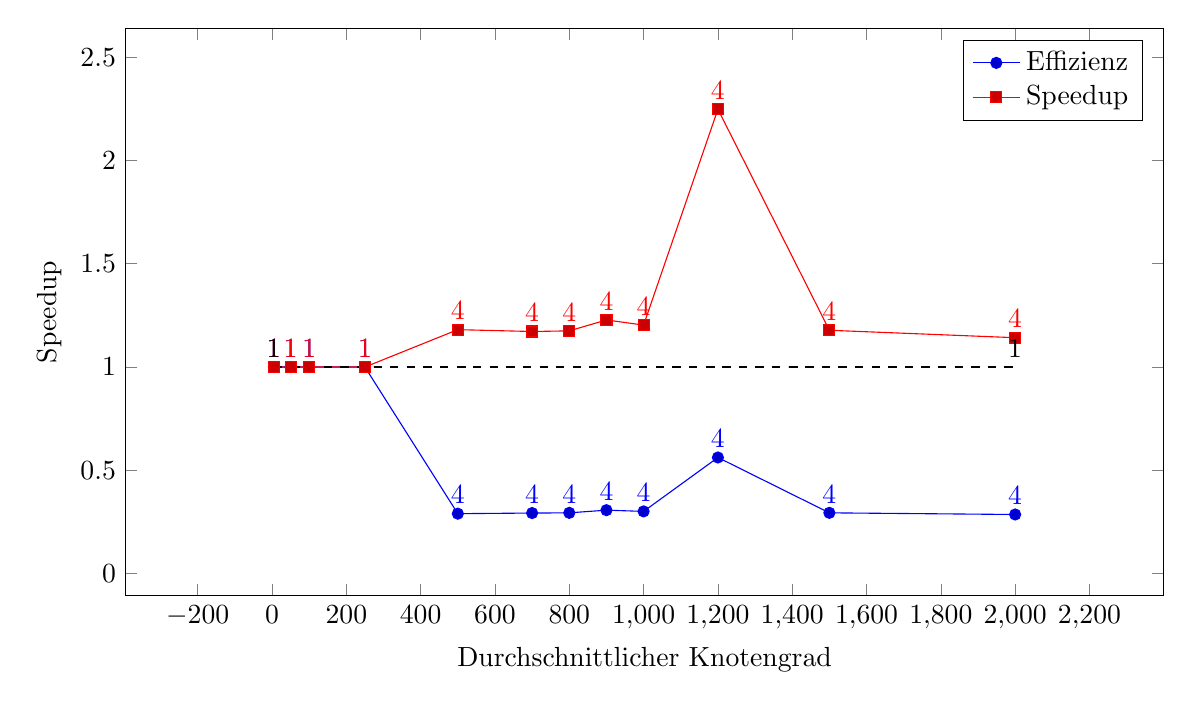
\begin{tikzpicture}
		\begin{axis}[nodes near coords,
			enlargelimits=0.2,
			width=420, height=250,
			xlabel=Durchschnittlicher Knotengrad,
	        ylabel=Speedup]

		    \addplot+[	        
		        point meta=explicit symbolic]
		    coordinates {
		        (5,1) [1]
		        (50,1) [1]
		        (100,1) [1]
		        (250,1) [1]
		        (500,0.29) [4]
		        (700,0.293) [4]
		        (800,0.294) [4]
		        (900,0.307) [4]
		        (1000,0.301) [4]
		        (1200,0.562) [4]
		        (1500,0.294) [4]
		        (2000,0.286) [4]
		    };
		    \addlegendentry{Effizienz}

		    \addplot+[
		        point meta=explicit symbolic]
		    coordinates {
		        (5,1) [1]
		        (50,1) [1]
		        (100,1) [1]
		        (250,1) [1]
		        (500,1.181) [4]
		        (700,1.172) [4]
		        (800,1.175) [4]
		        (900,1.228) [4]
			    (1000,1.203) [4]
			    (1200,2.248) [4]
			    (1500,1.178) [4]
			    (2000,1.142) [4]
			};
		    \addlegendentry{Speedup}

		    \addplot+[
		        smooth,
		        dashed,
		        black,
		        mark=none]
		    coordinates {
		    	(5,1)
		    	(2000,1)
		    };

		\end{axis}
	\end{tikzpicture}
\end{figure}

\begin{figure}
	\centering
	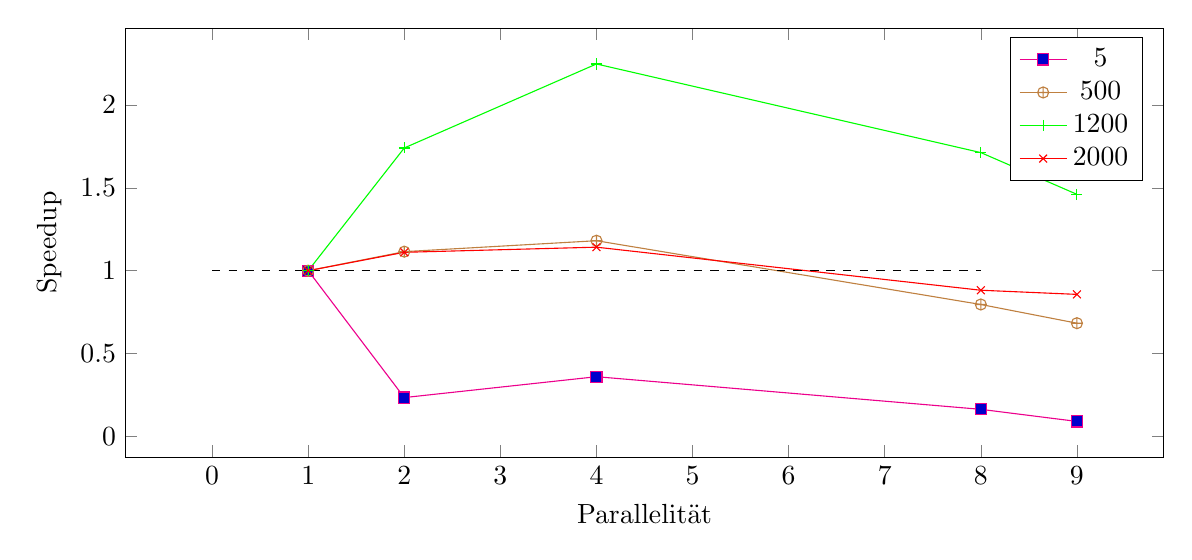
\begin{tikzpicture}
		\begin{axis}[
	        xlabel=Parallelität,
	        ylabel=Speedup,
	        width=420, height=200]

		    \addplot+[
		    magenta,
		    solid,
		    mark=square*]
		    coordinates {
		        (1,1)
		        (2,0.234)
		        (4,0.36)
		        (8,0.163)
		        (9,0.090)
		    };
		    \addlegendentry{5}

		    \addplot+[
		    brown,
		    solid,
		    mark=oplus]
		    coordinates {
		        (1,1)
		        (2,1.115)
		        (4,1.181)
		        (8,0.796)
		        (9,0.683)
		    };
		    \addlegendentry{500}

		    \addplot+[
		    green,
		    solid,
		    mark=+]
		    coordinates {
		        (1,1)
		        (2,1.741)
		        (4,2.248)
		        (8,1.713)
		        (9,1.461)
		    };
		    \addlegendentry{1200}

		    \addplot+[
		    red,
		    solid,
		    mark=x]
		    coordinates {
		        (1,1)
		        (2,1.111)
		        (4,1.142)
		        (8,0.882)
		        (9,0.857)
		    };
		    \addlegendentry{2000}

		    \addplot+[
		        smooth,
		        dashed,
		        black,
		        mark=none]
		    coordinates {
		    	(0,1)
		    	(8,1)
		    };

		\end{axis}
	\end{tikzpicture}
	\caption{Speedup des 1D-Algorithmus über Anzahl der Places. Die Dichte variiert. Als Referenzwert wurde jeweils der schnellste serielle Algorithmus genommen. Es wurden immer die schnellsten, gemessenen Werte verwendet.}
	\label{fig:verteilung_dichte}
\end{figure}
% subsection dichte (end)
%!TEX root = thesis.tex
\subsection{Verteilung} % (fold)
\label{sub:verteilung}
Die Ergebnisse der hier besprochen Testreihe, finden sich allesamt in Anhang \ref{Anhang-Messwerte-Verteilung}. Bei der Testreihe wurde die Knotenzahl fest auf 100 000 festgelegt und der durchschnittliche Kantengrad fest auf 750 eingestellt. Jeder Graph hat also auch die selbe absolute Kantenzahl. Diese Zahl wurde relativ hoch angesetzt, um genug Spielraum für die Variation der Verteilung zu haben. Ein Graph, dessen minimaler und maximaler Knotengrad weit vom durchschnittlichen Knotengrad entfernt ist, wird \textit{ungleichmäßig} genannt. Das Gegenteil dazu wird als \textit{gleichmäßig} bezeichnet. 

Zunächst fällt auf, dass die seriellen Laufzeiten in der Praxis konstant sind, wie es die Theorie vorhersagt. Dadurch ist in dieser Testreihe der Speedup besonders gut vergleichbar. In Abbildung \ref{fig:verteilung_speedup} ist die oberste Kurve der Speedup des gleichmäßigsten Graphen und die untere Kurve die, des ungleichmäßigsten Graphen. Es ist deutlich ersichtlich, dass das Parallelisierungspotential eines Graphen stark von der Verteilung der Knotengrade abhängt. Um so gleichmäßiger diese verteilt sind, um so besser funktioniert die Parallelisierung. Ein mögliche Erklärung ist, dass bei einem gleichmäßig verteilten Graph die Wahrscheinlichkeit größer ist, dass die Rechenlast gleichmäßig auf alle Places verteilt wird. Bei ungleichmäßigen Graphen hingegen, ist es eher zufällig, auf welchem Place wie viele aktive Knoten liegen. Auf die Größe der Datenmengen, die zwischen den Places transportiert werden muss, dürfte die Verteilung keinen Einfluss haben.

\begin{figure}
	\centering
	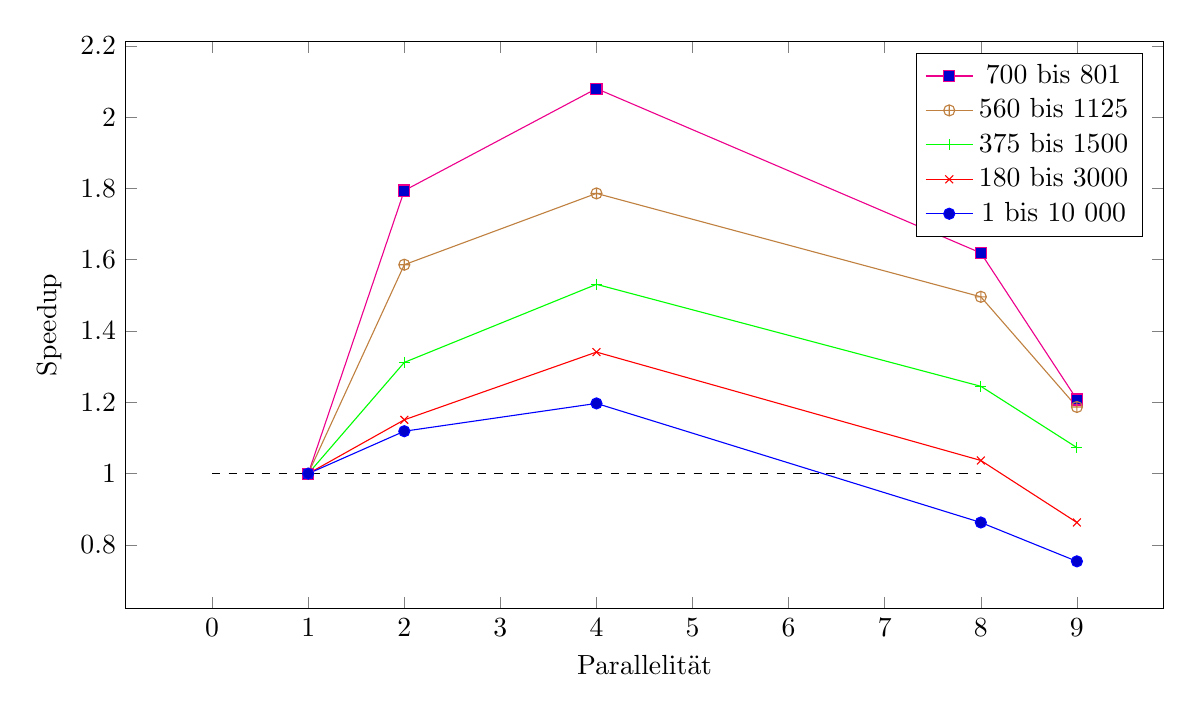
\begin{tikzpicture}
		\begin{axis}[
	        xlabel=Parallelität,
	        ylabel=Speedup,
	        width=420, height=250]

		    \addplot+[
		    magenta,
		    solid,
		    mark=square*]
		    coordinates {
		        (1,1)
		        (2,1.794)
		        (4,2.080)
		        (8,1.619)
		        (9,1.208)
		    };

		    \addlegendentry{700 bis 801}
		    \addplot+[
		    brown,
		    solid,
		    mark=oplus]
		    coordinates {
		        (1,1)
		        (2,1.586)
		        (4,1.786)
		        (8,1.496)
		        (9,1.187)
		    };
		    \addlegendentry{560 bis 1125}

		    \addplot+[
		    green,
		    solid,
		    mark=+]
		    coordinates {
		        (1,1)
		        (2,1.312)
		        (4,1.531)
		        (8,1.245)
		        (9,1.073)
		    };
		    \addlegendentry{375 bis 1500}

		    \addplot+[
		    red,
		    solid,
		    mark=x]
		    coordinates {
		        (1,1)
		        (2,1.151)
		        (4,1.341)
		        (8,1.037)
		        (9,0.863)
		    };
		    \addlegendentry{180 bis 3000}

		    \addplot+[
		    blue,
		    solid,
		    mark=*]
		    coordinates {
		        (1,1)
		        (2,1.119)
		        (4,1.197)
		        (8,0.863)
		        (9,0.754)
		    };
		    \addlegendentry{1 bis 10 000}

		    \addplot+[
		        smooth,
		        dashed,
		        black,
		        mark=none]
		    coordinates {
		    	(0,1)
		    	(8,1)
		    };

		\end{axis}
	\end{tikzpicture}
	\caption{Speedup des 1D-Algorithmus über Anzahl der Places. Die Verteilung variiert. Als Referenzwert wurde jeweils der schnellste serielle Algorithmus genommen. Pro Graph ist eine Kurve eingezeichnet. Es wurden immer die schnellsten, gemessenen Werte verwendet.}
	\label{fig:verteilung_speedup}

\end{figure}
% subsection verteilung (end)
%!TEX root = thesis.tex
\subsection{Größe} % (fold)
\label{sub:gr_e}
Die Testreihe, um die Auswirkung der Größe eines Graphen auf die Algorithmen herauszufinden, orientiert sich an einem Socialgraph. Es wurde geschätz, dass jeder durchschnittlich 100 Freunde hat, jeder mehr als einen Freund hat und keiner mehr als 500 Freunde hat. Das ergibt einen durchschnittlichen Knotengrad von 100, wobei der Knotengrad zwischen 1 und 500 liegt. Variiert wurde nun die Größe der Graphen. Es handelt sich hier um relativ dünn besetzte Graphen, so dass selbst der 500 000 Knoten Graph noch unter 500 MB liegt. Es wurde versucht, die Graphgröße weiter auf bis zu 2 Millionen Knoten zu steigern, was allerdings nicht möglich war. Graphen mit vielen Knoten resultieren in großen Sendepuffern und wie sich herausstellte, ist X10 dem nicht gewachsen. Der Sendevorgang (der \textit{at} Block) wird in den meisten fällen nie verlassen. Deswegen wurde hier die Knotenzahl auf 500 000 beschränkt. Es ist zu vermuten, dass diese Größe nicht ausreicht, um gute Ergebnisse bei der Parallelisierung zu erreichen.

Des weiteren wurde in dieser Testreihe der Modus mit 9 Places und der invasive Algorithmus weggelassen. Dass mit 9 Places auf 8 Kernen die Performance nicht gut sein wird, war bereits zu erwarten und bestätigte sich. Der invasive Algorithmus hatte ebenso Probleme mit der Graphgröße, was zwar durch Implementierungstricks umgangen werden könnte, aber allerdings den Zeitrahmen gesprengt hätte. Wieso der invasive Algorithmus nicht funktioniert, ist in der Bemerkung unten erläutert.

Bei jedem Graph dieser Testreihe war die serielle Version am schnellsten, was nach den vorangegangenen Ergebnissen auf keinen Fall zu erwarten war. Die serielle Version war schneller als jeder andere Algorithmus, egal mit wie vielen Places. Im Kapitel \ref{sub:dichte}, in dem die Dichte variierte, war der 1D-Algorithmus schon im Fall mit nur einem Place schneller, als der serielle Algorithmus. Da das hier nicht auftritt, ist zu vermuten, dass der 1D Algorithmus für dichte Graphen ein wenig schneller zu sein scheint, während der serielle Algorithmus für dünn besetzte Graphen schneller ist.
% TODO: Begründung? 

Vergleicht man nur den 1D-Algorithmus mit sich selbst bei steigender Anzahl an Places, zeichnet sich das Bild, dass 2 Places das Maximum zu sein scheint. In Abbilgun \ref{fig:groesse_speedup} ist sehr schön zu sehen, dass der Algorithmus mit 2 Places immer schneller war, als der Algorithmus mit 4 Places. Bei 8 Places war der Speedup immer kleiner als 1, was langsamere Laufzeit als die Referenzzeit bedeutet. Wie zu erwarten steigt tendenziell mit der Anzahl der Knoten das Parallelisierungspotential, wobei es durch den dünn besetzte Graph einigermaßen beschränkt zu sein scheint. Wäre dem nicht so müsste der Algorithmus auf 4 Places gegenüber den 2 Places aufholen, bei steigender Knotenzahl.

Für den 2D Algorithmus gilt, dass nie ein Speedup kleiner 1 erreicht wurde. Die hier verwendeten Graphen sind dafür zu klein.

\begin{figure}
	\centering
	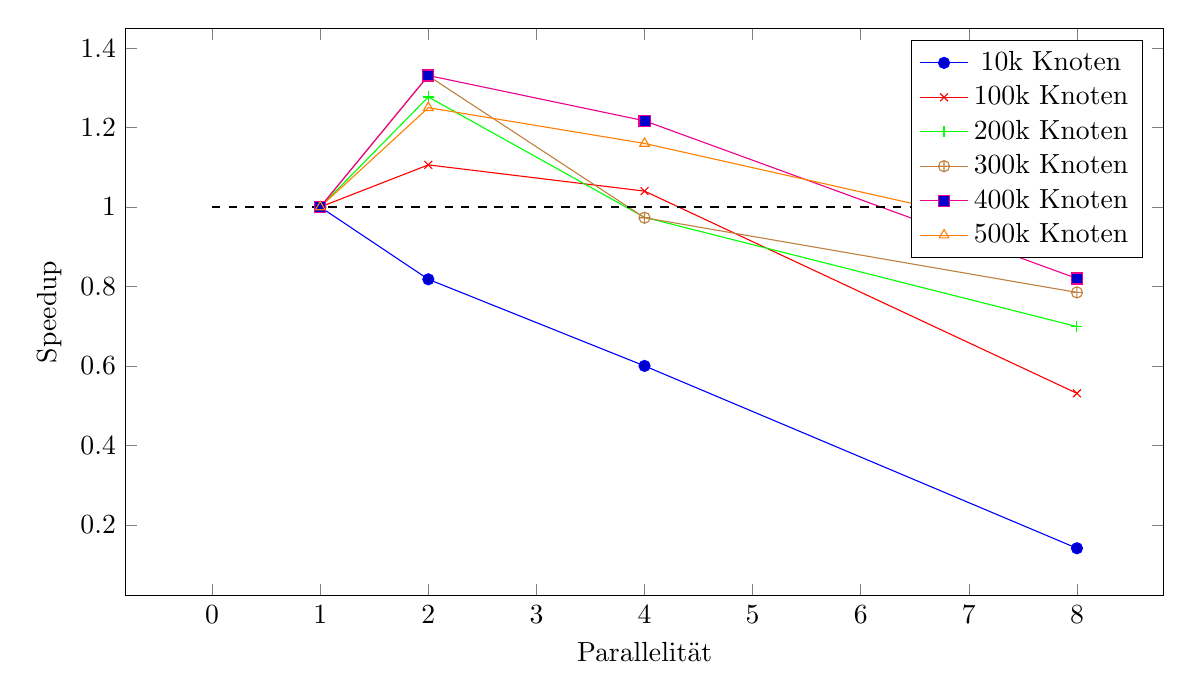
\begin{tikzpicture}
		\begin{axis}[
	        xlabel=Parallelität,
	        ylabel=Speedup,
	        width=420, height=250]

		    \addplot+[
		    blue,
		    solid,
		    mark=*]
		    coordinates {
		        (1,1)
		        (2,0.818)
		        (4,0.6)
		        (8,0.141)
		    };
		    \addlegendentry{10k Knoten}

		    \addplot+[
		    red,
		    solid,
		    mark=x]
		    coordinates {
		        (1,1)
		        (2,1.106)
		        (4,1.04)
		        (8,0.531)
		    };
		    \addlegendentry{100k Knoten}

		    \addplot+[
		    green,
		    solid,
		    mark=+]
		    coordinates {
		        (1,1)
		        (2,1.277)
		        (4,0.974)
		        (8,0.699)
		    };
		    \addlegendentry{200k Knoten}

		    \addplot+[
		    brown,
		    solid,
		    mark=oplus]
		    coordinates {
		        (1,1)
		        (2,1.330)
		        (4,0.973)
		        (8,0.785)
		    };
		    \addlegendentry{300k Knoten}

		    \addplot+[
		    magenta,
		    solid,
		    mark=square*]
		    coordinates {
		        (1,1)
		        (2,1.331)
		        (4,1.217)
		        (8,0.82)
		    };
		    \addlegendentry{400k Knoten}

		    \addplot+[
		    orange,
		    solid,
		    mark=triangle]
		    coordinates {
		        (1,1)
		        (2,1.25)
		        (4,1.16)
		        (8,0.916)
		    };
		    \addlegendentry{500k Knoten}

		    \addplot+[
		        smooth,
		        dashed,
		        black,
		        mark=none]
		    coordinates {
		    	(0,1)
		    	(8,1)
		    };

		\end{axis}
	\end{tikzpicture}
	\caption{Speedup des 1D-Algorithmus über Anzahl der Places. Variiert wurde die Größe des Graphen. Als Referenzwert wurde jeweils der 1D-Algorithmus mit einem Place genommen. Eine Kurve pro Graph.}
	\label{fig:groesse_speedup}
\end{figure}

\underline{Bemerkung:}
Beim Parsen der Graphdatei gehen alle Implementierungen so vor, dass sie Zeile für Zeile in die Datenstruktur eingepflegt werden. Dabei steht schon vor dem Parsen fest, welches Datum auf welchen Place muss. Die Informationshäppchen, die von Place zu Place übertragen werden müssen, sind relativ klein. Im invasiven Fall ergibt es wenig Sinn, schon ein \textit{invade} aufzurufen, bevor überhaupt der Graph eingelesen wurde, bevor also die Größe des Problems bekannt ist. Aus diesem Grund wird der Graph erst lokal auf den ersten Place eingelesen, dann der Constraint zusammengebaut und erst wenn der Claim bekannt ist, auf die involvierten Places verteilt. Die hier zu übetragenen Daten sind relativ groß, womit X10 Probleme zu haben scheint. Das Problem könnte umgangen werden, indem die Datenstruktur in kleinere Häppchen aufgeteilt wird. Das ist aber höchstens ein Workaround um ein Problem, das bei X10 liegt.
% subsection gr_e (end)

% section ergebnisse_der_parallelisierung (end)

\section{Die 2D Breitensuche} % (fold)
\label{sec:die_2d_breitensuche}
Die 2D Breitensuche ist in jedem Testfall der mit Abstand langsamste Algorithmus gewesen, was so nicht zu erwarten war. Der implementierte Algorithmus ist zwar zunächst deutlich komplexer, als die anderen beiden, doch gibt es zwei Vorteile, die diesen Algorithmus gewiss studierenswert machen. Erstens sind die Gruppen von Places, die untereinander kommunizieren deutlich kleiner. In der ersten Kommunikationsphase sendet jeder Place seine Daten an eine ganze Spalte, und empfängt dafür von einer ganzen Zeile die Daten für den nächsten Schritt. Das sind $2 * \sqrt(p)$ Places, insgesamt, mit denen jeder Place kommunizieren muss, also $O(p * 2 + \sqrt(p) * \frac{1}{2}) = O(p * \sqrt(p))= O(p^{\frac{3}{2}})$ Kommunikationsvorgänge im System. In der zweiten Kommunikationsphase muss jeweils nur eine Zeile miteinander kommunizieren. Das sind zusätzlich $O(\sqrt(p) * p * \frac{1}{2})$ Kommunikationsvorgänge. Es sind also im O-Kalkül pro Iteration $O(p^{\frac{3}{2}})$. Im Vergleich dazu kommuniziert jeder Place im 1D Algorithmus mit allen anderen p-1 Places, also $O(p^2)$ Kommunikationsvorgänge. Der zweite Vorteil der Implementierung wie in \cite{Buluc:2011} ist die Möglichkeit, alle Kommunikation und Synchronisation auf drei MPI Operationen abzubilden. Die auf entsprechender Hardware vergleichsweise schnell sind. 

Beide dieser Vorteile sind bei der X10 Implementierung, die auf nur einem CPU läuft, hinfällig. Zunächst wurden die MPI Operationen in X10 \enquote{nachprogrammiert}. Um das zu tun, muss \textit{at} verwendet werden, dass einen für diesen Zweck unnützen Rückkanal bereithält, der zusätzliche Latenz in jede Kommunikation bringt. Weiterhin gibt es bei der Verwendung einer hochperformanten MPI Hardware den Vorteil, dass ein Datum nur einmal gesendet werden muss, wenn es an mehrere Empfänger gehen soll. Das ist in X10-Syntax nicht möglich. Die zusätzliche Kommunikation ist also teurer, als sie sein müsste. 
Der zweite Vorteil, eben dass weniger Kommunikationsvorgänge im System sind, ist aus zwei Gründen hier nicht ausschlaggebend. Zum einen sind dermaßen wenig Places im Spiel, dass es kaum einen Unterschied zwischen $O(p^{\frac{3}{2}})$ und $O(p^2)$ gibt, zum anderen haben erste Tests gezeigt, dass die Kommunikationsphasen etwa 4 bis 5 Mal so schnell sind wie die Rechenphasen, also die Kommunikation nicht so ausschlaggebend ist, wie das zu erwarten war. Das wiederum ist auf die Testumgebung ohne wirklich getrennte Places zurückzuführen.

Wie in \cite{Buluc:2011} ist also auch in X10 die 2D Implementierung eher die schlechtere, wobei in den Dimensionen, in denen in dieser Arbeit gedacht wird, die Unterschiede gravierender sind. Ob in größeren Testumgebungen die Ergebnisse anders ausfallen, muss in einer weiteren Arbeit untersucht werden.
% section die_2d_breitensuche (end)

\section{Invasive Breitensuche} % (fold)
\label{sec:invasive_breitensuche}
Im Rahmen dieser Arbeit wurden Ansätze herausgearbeitet, um die Breitensuche an das invasive Rechnen im Allgemeinen und an das Framework invadeX10 im Speziellen, anzupassen. Die Ergebnisse fielen dabei zwar besser aus, als erwartet, doch sind die Laufzeiten immernoch erheblich länger, als die der 1D Breitensuche. Die benötigte Zeit zur Lösung einer BFS-Instanz zu vergleichen wäre unfair und nicht zielführend, weswegen darauf gänzlich verzichtet wird. Die Intention des invasiven Rechnens war es nie, eine einzelne Instanz möglichst schnell zu lösen. Um einen fairen Vergleich durchzuführen, müsste eine Menge von verschiedenen Jobs und eine Zielhardware definiert werden. Daraufhin muss verglichen werden, wie lange es mit verschiedenen Strategien braucht, bis alle Jobs erledigt wurden. Die Strategien sind zum Beispiel, alle gleichzeitig starten, ein Job nach dem anderen starten oder eben invasives Vorgehen. In Mangel der invasiven Hardware und ausgereiften Softwareinstrumenten um diese zu simulieren, musste darauf in dieser Arbeit verzichtet werden. Die Ergebnisse sind aber insofern nicht schlecht, als dass sie nur 3 - 5 mal so langsam sind, wie die schnellsten Laufzeiten. Außerdem profiert auch die invasive Breitensuche, die sehr viel overhead hat, von den Parallelisierung auf mehrere Places.
% section invasive_breitensuche (end)

\section{Wikipedia und die Philosophie} % (fold)
\label{sec:wikipedia_und_die_philosophie}
Der bekannte Webcomic xkcd stellt die Behauptung auf, wenn man in der Wikipedia wiederholt auf den ersten Link klickt (der nicht in Klammern steht), gelangt man irgendwann zu dem Arikel über Philosphie \cite{xkcd:Online}. Im Rahmen dieser Arbeit wurde die deutsche Wikipedia heruntergeladen, zu einem Graph verarbeitet und mittels Breitensuche herausgefunden,
\begin{enumerate}
	\item dass diese Behauptung für ca. 42\% der Artikel wahr ist,
	\item dass man durchschnittlich 5,52 mal klicken muss, um zum Artikel \enquote{Philosphie} zu gelangen, falls das denn möglich ist,
	\item dass es einen Zykel gibt: Philosphie $\rightarrow$ Wissenschaft $\rightarrow$ Wissen $\rightarrow$ Erkenntnistheorie $\rightarrow$ Philosphie. Punkt 1 gilt also für alle vier Wikipediaartikel
	\item und dass die Wissenschaft noch \enquote{zentraler} in der Wikipedia ist. Die durchschnittliche Klickanzahl ist hier bei nur 4,49.
\end{enumerate}
Den eigentlichen Zweck des Graphs, nämlich als Testdatum zu fungieren, konnte er leider nicht erfüllen, da er einfach zu klein ist, um sich für die Parallelisierung zu eignen.
% section wikipedia_und_die_philosopie (end)
% chapter ergebnisse_und_diskussion (end)